


\begin{figure}

    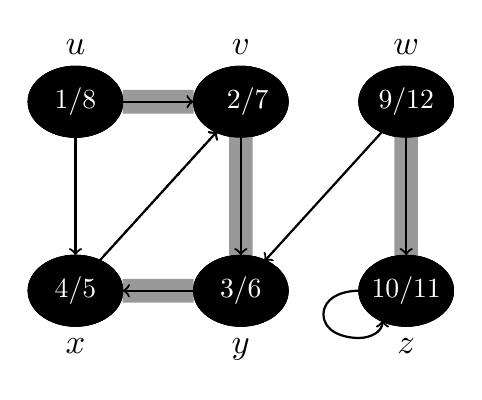
\begin{tikzpicture}[scale=.3]
    \centering
    
        %\draw [ultra thick,help lines] (-10,-5) grid(10,10);
        
       %\draw [line width=.3pt] (-10,0) -- (10,0); %x axis
        %\draw [line width=.3pt] (0,-5) -- (0,10); % y axis
        
        
        \draw (-7,7) ellipse (2cm and 1.5cm);  %u
        \draw (0,7) ellipse (2cm and 1.5cm); %v
        \draw (7,7) ellipse (2cm and 1.5cm); %w
        \draw  (-7,-1) ellipse (2cm and 1.5cm); %x
        \draw  (0,-1) ellipse (2cm and 1.5cm); %y
        \draw (7,-1) ellipse (2cm and 1.5cm); %z
        
   
        
        
        
        \node [above,scale=1.25] at(-7,8.5) {$\displaystyle{u}$};
        \node [above,scale=1.25] at(0,8.5) {$\displaystyle{v}$};
        \node [above,scale=1.25] at(7,8.5) {$\displaystyle{w}$};
        \node [below,scale=1.25] at(-7,-2.5) {$x$};
        \node [below,scale=1.25] at(0,-2.5) {$\displaystyle{y}$};
        \node [below,scale=1.25] at(7,-2.5) {$\displaystyle{z}$};
        
       
        
        
        %\draw [line width=.5pt,->] (-7,5.5) -- (-7,.5);
        \draw [<-=latex,->=latex,thick] (-7,5.5) -- (-7,.5); %u to x
        \draw [<-=latex,->=latex,thick] (-5,7) -- (-2,7); % u to v
        
        
        \draw [<-=latex,->=latex,thick] (0,5.5) -- (0,.5); % v to y
        
        \draw [<-=latex,->=latex,thick] (7,5.5) -- (7,.5); % w to z
        \draw [<-=latex,->=latex,thick] (6,5.75) -- (1,.25);% w to y
        
        \draw [<-=latex,->=latex,thick] (-6,.25) -- (-1,5.75);% x to v
        
        \draw [<-=latex,->=latex,thick] (-2,-1) -- (-5,-1); % y to x
        
       % \draw [<-=latex,->=latex,thick] (5,-1) to [out=180,in=-90] (6,-2.2);
       
       \draw [->=latex,thick] (5,-1) to [out=180,in=90] (3.5,-2) to [out=-90,in=-180] (5,-3) to [out=0,in=-90] (6,-2.25);\pause
       
       
        
       
       % picture a 
       \draw[fill=gray!50] (-7,7) ellipse (2cm and 1.5cm); %u is gray
        \node[above,scale=1] at(-7,6) {\textcolor{black}{1/}}; \pause
        
        
        
        %picture b
        \draw[fill=gray!50] (0,7) ellipse (2cm and 1.5cm); %v is gray
        \node[above,scale=1] at (0,6) {2/};
        \path[fill=gray!80] (-5,6.5) -- (-5,7.5) -- (-2,7.5) -- (-2,6.5) -- (-5,6.5);
        \draw [<-=latex,->=latex,thick] (-5,7) -- (-2,7); \pause % u to v
        
        
        %picture c
        \draw[fill=gray!50]  (0,-1) ellipse (2cm and 1.5cm); %y is gray
         \node[below,scale=1] at (0,0) {3/};
          \path[fill=gray!80] (-.5,0.5) -- (-.5,5.5) -- (.5,5.5) -- (.5,0.5) -- (-.5,0.5);
          \draw [<-=latex,->=latex,thick] (0,5.5) -- (0,.5); \pause  % v to y
          
          %picture d
          \draw[fill=gray!50]  (-7,-1) ellipse (2cm and 1.5cm); %x is gray
          \node[below,scale=1]  at (-7,0) {4/};
           \path[fill=gray!80] (-2,-.5) -- (-2,-1.5) -- (-5,-1.5) -- (-5,-.5) -- (-2,-.5); 
          \draw [<-=latex,->=latex,thick] (-2,-1) -- (-5,-1);\pause % y to x
          
          %picture e
          \draw [<-=latex,->=latex,thick,dotted] (-6,.25) -- (-1,5.75); \pause % x to v
          
          %picture f
          \draw[fill=black]  (-7,-1) ellipse (2cm and 1.5cm); %x is black
          \node[below,scale=1]  at (-7,0) {\textcolor{white}{4/5}};\pause
          
          %picture g
          \draw[fill=black]  (0,-1) ellipse (2cm and 1.5cm); %y is black
          \node[below,scale=1] at (0,0) {\textcolor{white}{3/6}};\pause
          
         %picture h
         \draw[fill=black] (0,7) ellipse (2cm and 1.5cm); %v is black
         \node[above,scale=1] at (0,6) {7\textcolor{white}{2/7}};\pause
         
         
         %picture j
         \draw[fill=black] (-7,7) ellipse (2cm and 1.5cm); %u is black
         \node[above,scale=1] at(-7,6) {\textcolor{white}{1/8}}; \pause
         
         %picture k
         \draw[fill=gray!50] (7,7) ellipse (2cm and 1.5cm);  %w is gray
         \node[above,scale=1] at (7,6) {9/}; \pause
         
         %picture l
         
         %picture m
         \draw[fill=gray!50] (7,-1) ellipse (2cm and 1.5cm); %z is gray
         \node[below,scale=1] at (7,0) {10/};
         \path[fill=gray!80] (6.5,.5) -- (6.5,5.5) -- (7.5,5.5) -- (7.5,.5) -- (6.5,.5);
         \draw [<-=latex,->=latex,thick] (7,5.5) -- (7,.5); \pause % w to z
         
         % picture n
         
         %picture o
         \draw[fill=black] (7,-1) ellipse (2cm and 1.5cm); %z is black
         \node[below,scale=1] at (7,0) {\textcolor{white}{10/11}};\pause
         
         %picture p
         \draw[fill=black] (7,7) ellipse (2cm and 1.5cm);  %w is black
         \node[above,scale=1] at (7,6) {\textcolor{white}{9/12}};
         
         
        
    
    \end{tikzpicture}

\end{figure}

